%last updated in April 2002 by Antje Endemann

\documentclass[runningheads]{llncs}
%In order to omit page numbers and running heads
%please use the following line instead of the first command line:
%\documentclass{llncs}.
%Furthermore change the line \pagestyle{headings} to
%\pagestyle{empty}.
\usepackage{graphicx}
\usepackage{url}
\usepackage{color}
\usepackage{amsmath}
\newcommand{\argmin}{\operatornamewithlimits{argmin}}
\newcommand {\afbnote} [1] {{\bf \textcolor{red}{(#1)}}}
\newcommand {\ericnote} [1] {{\bf \textcolor{magenta}{(#1)}}}
\newcommand {\PnP} {P$n$P}
\newcommand {\EPnP} {EP$n$P}
\input{psfig.sty}

\begin{document}

\pagestyle{headings}
%In order to omit page numbers and running heads
%please change this line to
%\pagestyle{empty}
%and change the first command line too, see above.

\mainmatter

\title{Camera pose from face images}

\titlerunning{Camera pose from face images}

\maketitle

\begin{abstract}
\afbnote{todo...}
\end{abstract}

\section{Introduction}
When photographing a human head, the subject's appearance can vary dramatically depending on the camera's distance from the subject.
This variation is caused by perspective distortion, and for 3D objects cannot be undone by simply adjusting focal length; see Figure \ref{fig:fiducial_migration} for an illustration using a synthetic head\footnote{Generated using FaceGen (\url{http://www.facegen.com}).}.

This distortion is evidently a problem for automatic cross-condition face recognition, e.g. webcam-based recognition from social media images.
Even humans find such recognition difficult \cite{liu2003face,liu2006face}.
It is also a source of information, allowing camera pose estimation in cases where the subject is known \cite{ohayon2006robust}.
This information could potentially be used to undistort the images and improve recognition results.

In this paper, we show camera distance estimation from 2D images is possible even when the subject is previously unseen.
Our technique replaces the known-subject assumption with knowledge of the general distribution of fiducials across people.
This distribution turns out to be sufficiently tight to allow precise distance estimation using only a small training set.

The paper is organized as follows.
Section \ref{sec:related} covers related work from psychology and computer vision.
Section \ref{sec:method} explains our method.
In Section \ref{sec:experiments}, we validate our method on the Texas 3D Face Recognition Database.
Section \ref{sec:discussion} is the discussion.

\begin{figure}[ht!]
\centering
\begin{tabular}{ccc}
\includegraphics[width=.33\linewidth]{resources/figures/extracted_fiducial_0006.png} &
\includegraphics[width=.33\linewidth]{resources/figures/extracted_fiducial_0008.png} &
\includegraphics[width=.33\linewidth]{resources/figures/extracted_fiducial_0001.png} \\
\includegraphics[width=.33\linewidth]{resources/figures/extracted_fiducial_0002.png} &
\includegraphics[width=.33\linewidth]{resources/figures/extracted_fiducial_0003.png} &
\includegraphics[width=.33\linewidth]{resources/figures/extracted_fiducial_0004.png} \\
\includegraphics[width=.33\linewidth]{resources/figures/extracted_fiducial_0005.png} &
\includegraphics[width=.33\linewidth]{resources/figures/extracted_fiducial_0007.png} &
\includegraphics[width=.33\linewidth]{resources/figures/fiducial_migration.png}
\end{tabular}
\caption{
\ericnote{TODO: Label each image with its camera distance.}
A synthetic head viewed from different camera distances, illustrating projective distortion.
Camera distance decreases in the first eight images, indexed in row-major order.
Here, the focal length (zoom) is adjusted to keep the figure at a constant size.
Fiducials are shown as red dots.
In the first image, the camera is a far distance, resulting in near orthographic projection.
In the eighth image (bottom row, middle column) the camera is very close to the human head, resulting in an elongated face and protruding nose.  
The last image is the same as the first, but with fiducial markers from all images.
This illustrates the migration of fiducials as a function of camera distance. 
} 
\label{fig:fiducial_migration}
\end{figure}

\subsection{Related works} \label{sec:related}
There is previous work on head pose estimation from 2D images; see \cite{murphy2009head} for a recent survey.
However, most methods attempt to recover a subset of the yaw, pitch, and roll of the head with respect to the camera.
To our knowledge, these methods do not attempt to estimate the distance between the camera and head; Figure \ref{fig:head_pose} illustrates the difference.
In this section we discuss works most similar to our own.

\begin{figure}[ht]
\centering
\includegraphics[width=1.0\linewidth]{resources/figures/head_pose.png}
\caption{
An illustration of the six degrees of freedom governing head pose relative to a camera.
Prior work has focused on estimation of yaw, pitch, and roll \cite{murphy2009head}.
In this paper, we assume these parameters are known and estimate camera distance from the subject, shown here as distance along the $z$ axis.
}
\label{fig:head_pose}
\end{figure}

In \cite{liu2003face,liu2006face}, Liu studies the effect of face recognition by humans when viewing faces at different perspective convergence angles (effectively focal length or field of view). 
The study involved a training phase in which face images were displayed to a human test subject.
In a later recognition phase the subject was shown images of faces and asked to determine whether each face had been previously displayed.
The field of view was changed to see if this had an effect on recognition. 
Their results show that even humans have a hard time recognizing a face when viewed under different levels of perspective distortion.  
This is a motivating factor since if human have trouble with this task, a computer vision algorithm will likely also have the same troubles.  
Predicting the distance between camera and face is a first step in mitigating the effects of perspective distortion.

A similar psychology based studied is presented in \cite{perona2007new,bryan2012perspective}. 
Here, Perona et al. investigate the effects of perspective distortion as visual cue for social judgement of faces.  
Human subjects were asked to judge an image of a face in terms of trustworthiness, attractiveness, and competence.  
Their results show that for social judgements, pictures taken from a distance inside personal space (up close) are generally rated lower, while pictures taken at a far distance have higher ratings.

In automatic camera calibration, camera parameters are recovered using prior information about the imaged scene.
In \cite{deutscher}, Deutscher et al. recover camera parameteres under the assumption the scene satisfies a Manhattan world criterion.
This is similar to our technque, which assumes human fiducial locations are approximately distributed according to an estimated distribution. 
In \cite{lv2006}, Lv et al. use a human subject for calibration, but unlike this work requires multiple frames of video.

In \cite{ohayon2006robust}, Ohayon and Rivlin present head tracking as a camera pose estimation problem.  
Prior to head tracking, 3D points are acquired from the head.  
During tracking, correspondences between the 3D points and their imaged 2D points are used to estimate head pose by solving the inverse problem, namely camera pose. 
They use the Perspective $n$-Point (\PnP) formulation to solve for the camera extrinsic parameters (rotation $R$ and translation $T$).  
The \PnP method is also known as the Location Determination Problem and was first coined in \cite{ransac}.  
In effect, the human head is used as a calibration rig.  
In this paper, the authors show that head pose can be accurately estimated and tracked under varying yaw, pitch, and roll and translations about $x$ and $y$ axes. 
However, they assume knowledge of the ground-truth fiducial locations and do not address dramatic changes in camera distance.

\section{Camera pose estimation from face images using \EPnP}

Our work is based on \cite{ohayon2006robust}, but we focus primarily on translation along the $z$-axis, which affects the level of induced perspective distortion.  
% Furthermore, Ohayon and Rivlin present a method for estimating head pose of a specific human head.  
We present a method for estimating the pose of a previously unseen human head using a dataset of exemplar human heads. 

\subsection{Efficient Perspective $n$-Point (\EPnP)}
\EPnP is a non-iterative solution to the \PnP problem.  
As stated earlier, the \PnP problem estimates the pose of a calibrated camera from $n$ 3D-to-2D correspondences.  
The advantage of \EPnP is that the computational complexity grows linearly with $n$, whereas other state-of-the-art methods are $O(n^5)$ or even $O(n^8)$.  
We use Matlab code provided by the authors \footnote{\url{http://cvlab.epfl.ch/software/EPnP}}.

\subsection{Exemplar 3D heads}
The geometric configuration of fiducial features does vary from face to face, but in general fiducial locations tend to form clusters, as illustrated in Figure \ref{fig:fiducial_clusters}.  
Figure \ref{fig:fiducial_clusters}(a-c) shows point clouds of three different faces taken from the GavaBDB \cite{moreno2004gavabdb} dataset. 
Manually clicked fiducial locations are marked with large red dots.
\ericnote{Descriptions for how to interpret figures should be moved to captions.}
Figure \ref{fig:fiducial_clusters}(c) shows fiducials for 20 different faces, note the fiducials form clusters.  
We take advantage of this and use a set of exemplar 3D heads to estimate the camera pose (in particular distance between camera and head) of face images in general. 
We show that using exemplar heads allows us to accurately estimate the camera pose and distance from camera to the head.

\begin{figure}[h]
\centering
\begin{tabular}{cc}
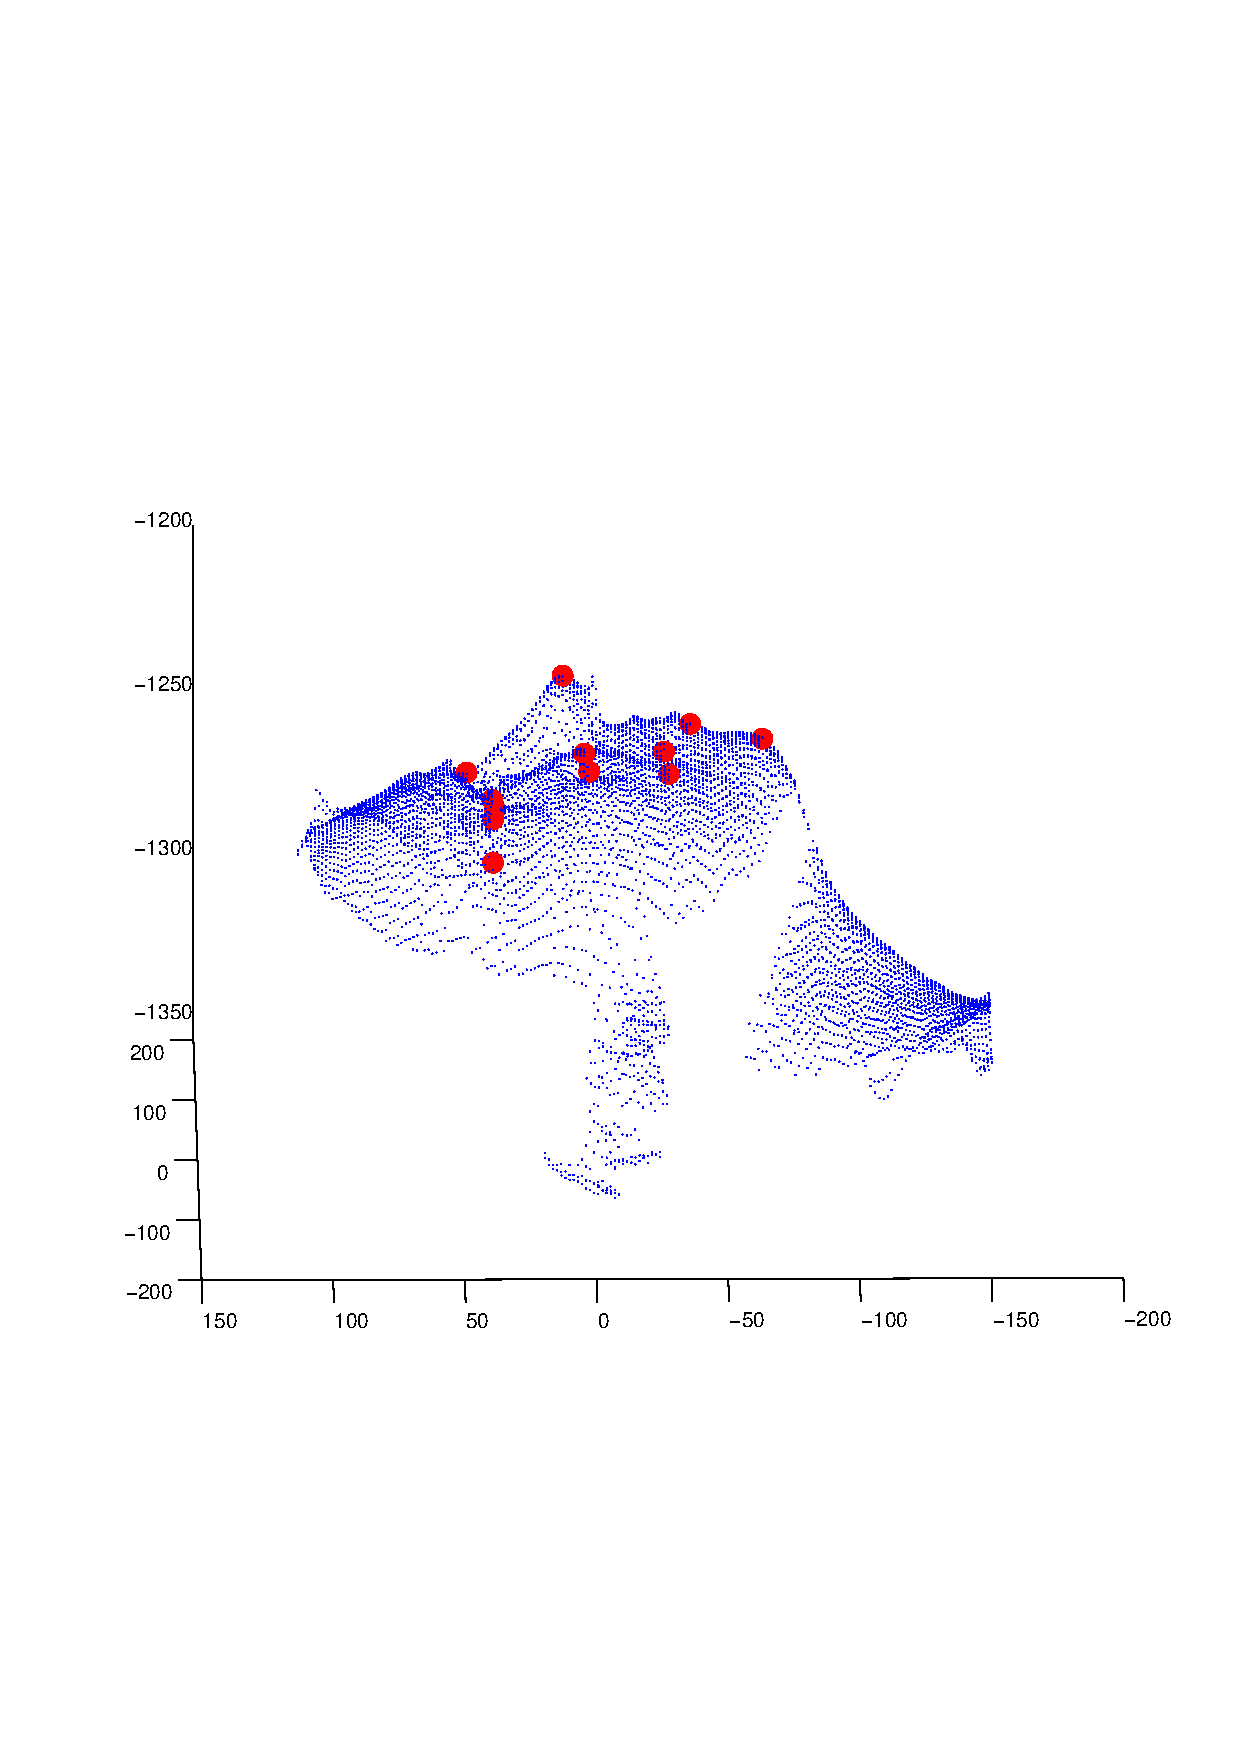
\includegraphics[width=.3\linewidth]{resources/figures/face1.png} &
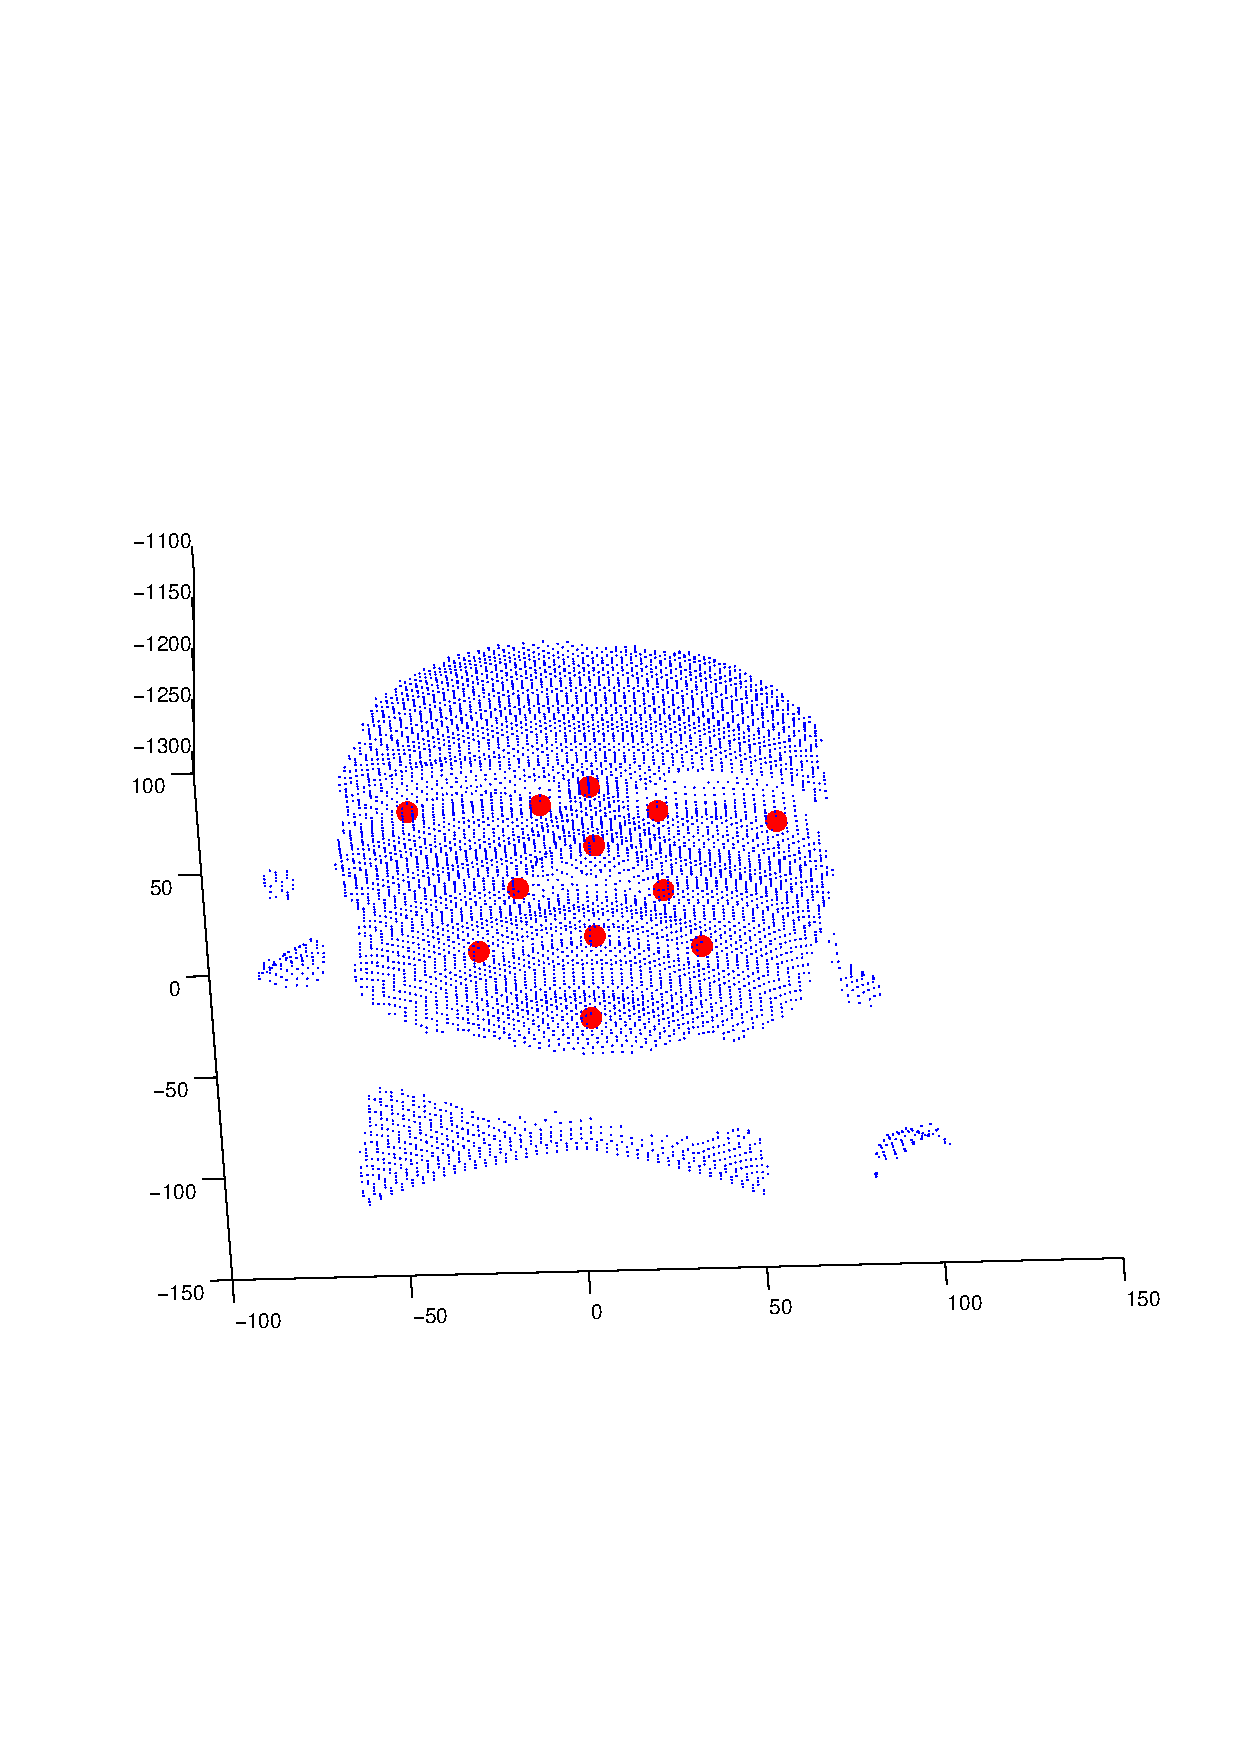
\includegraphics[width=.3\linewidth]{resources/figures/face2.png} \\
(a) & (b) \\
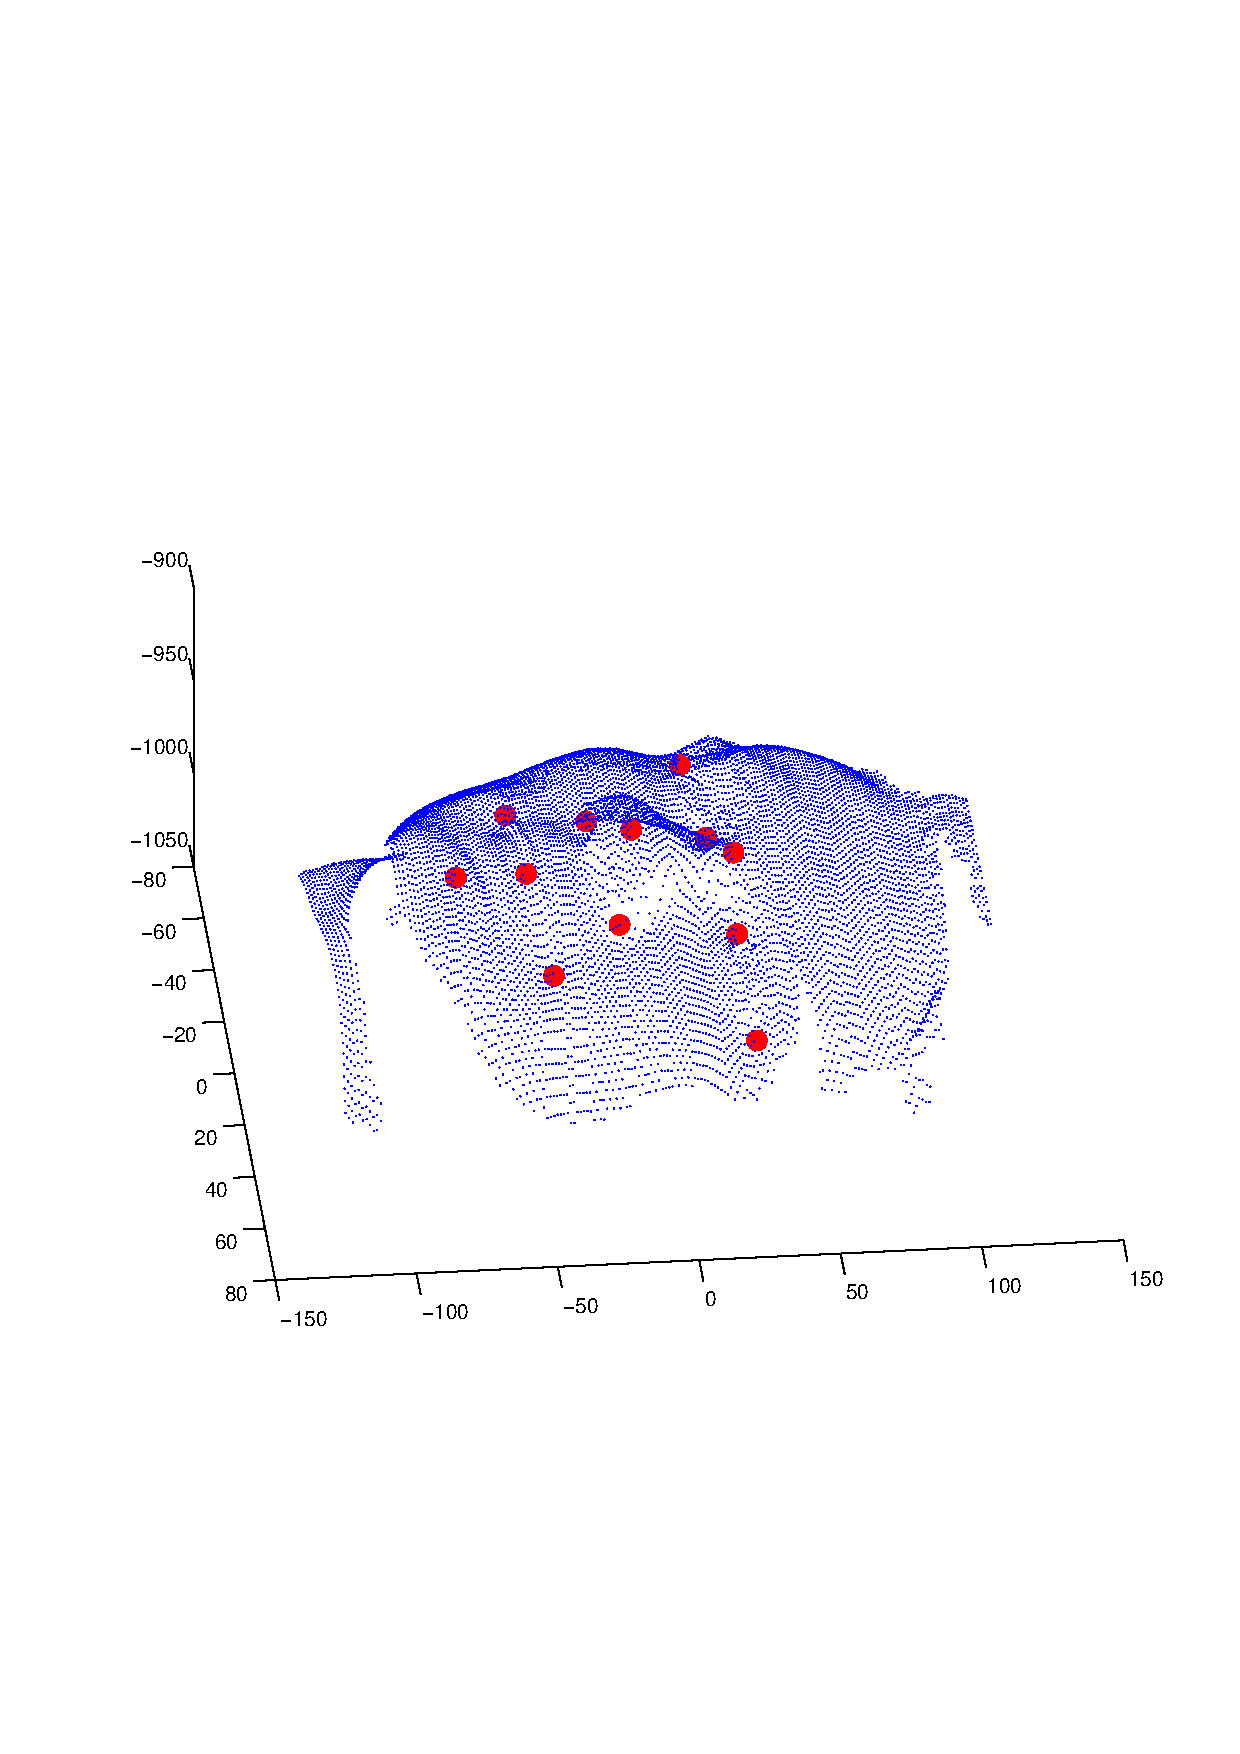
\includegraphics[width=.3\linewidth]{resources/figures/face3.png} &
\includegraphics[width=.5\linewidth]{resources/figures/fiducial_clusters.png} \\
(c) & (d)
\end{tabular}
\caption{(a-b) 3D point clouds of three different faces along with manually clicked fiducials.  (c) Fiducials from 20 faces.}
\label{fig:fiducial_clusters}
\end{figure}

\section{Experimental setup}
In all experiments, we use the Texas 3D Face Recognition Database (Texas 3DFRD) \cite{gupta2010texas}, see figure \ref{fig:t3dfrd}.  
This database is a collection of 1149 pairs of frontal facial color and range images of 105 adult human subjects.  
Each face also has 25 manually labeled anthropometric facial fiducial points.  
Color and range images were captured simultaneously and are thus perfectly registered to each other.  
This allows us to have ground truth 3D locations of the fiducial locations.  
\begin{figure}[h]
\centering
\includegraphics[width=.7\linewidth]{resources/figures/t3dfr.jpg}
\caption{Example images from the Texas 3DFRD.}
\label{fig:t3dfrd}
\end{figure}
In this work, we are primarily interested in recovering the distance between camera and head.  Our experiments consist of the following:

\begin{itemize}
\item Project fiducials for a test individual onto an image plane.
\item Use 3D fiducial locations for other individuals as exemplars.
\item For each exemplar, estimate the camera pose (and distance) using \EPnP.
\item Final estimate is the average from all exemplars.
\item Repeat while simulating a dolly-zoom camera movement (move camera back, increase focal length).  
\end{itemize}

We perform this experiment for the frontal and $3/4$ profile view of the face.  
For the frontal case, we assume all fiducials are visible to the camera.  
For the $3/4$ we assume only a subset of the fiducials are visible. 
In this work, we assume we have a calibrated camera and all intrinsic camera parameters are known.  
Simulated camera distances range from approximately 10cm to 300cm.

Note the distance of camera to the face could be trivially estimated by the size of the imaged face if we did not adjust the focal length. 
The focal length is adjusted to keep the outermost fiducials at a near constant distance, which also keeps the imaged face silhouette at a constant size.

Figure \ref{fig:results} shows results of camera pose estimation and distance from camera to head for the frontal and $3/4$ profile views.  Figure \ref{fig:results} (a,c) qualitatively show the estimated camera pose.  The true and estimated camera distances (Figure \ref{fig:results}(b,d) )represent the distance between the camera center and tip of the nose.  The distance is reported in centimeters using an estimate for the average distance between outermost fiducial markers ($12$ cm). Note the final distance estimate closely follows the true camera distance, though the error bars get larger as the distance increases.  This is specially true for the $3/4$ profile view, presumably due to fewer number of visible fiducials.   
\begin{figure}[ht]
\begin{tabular}{cc}
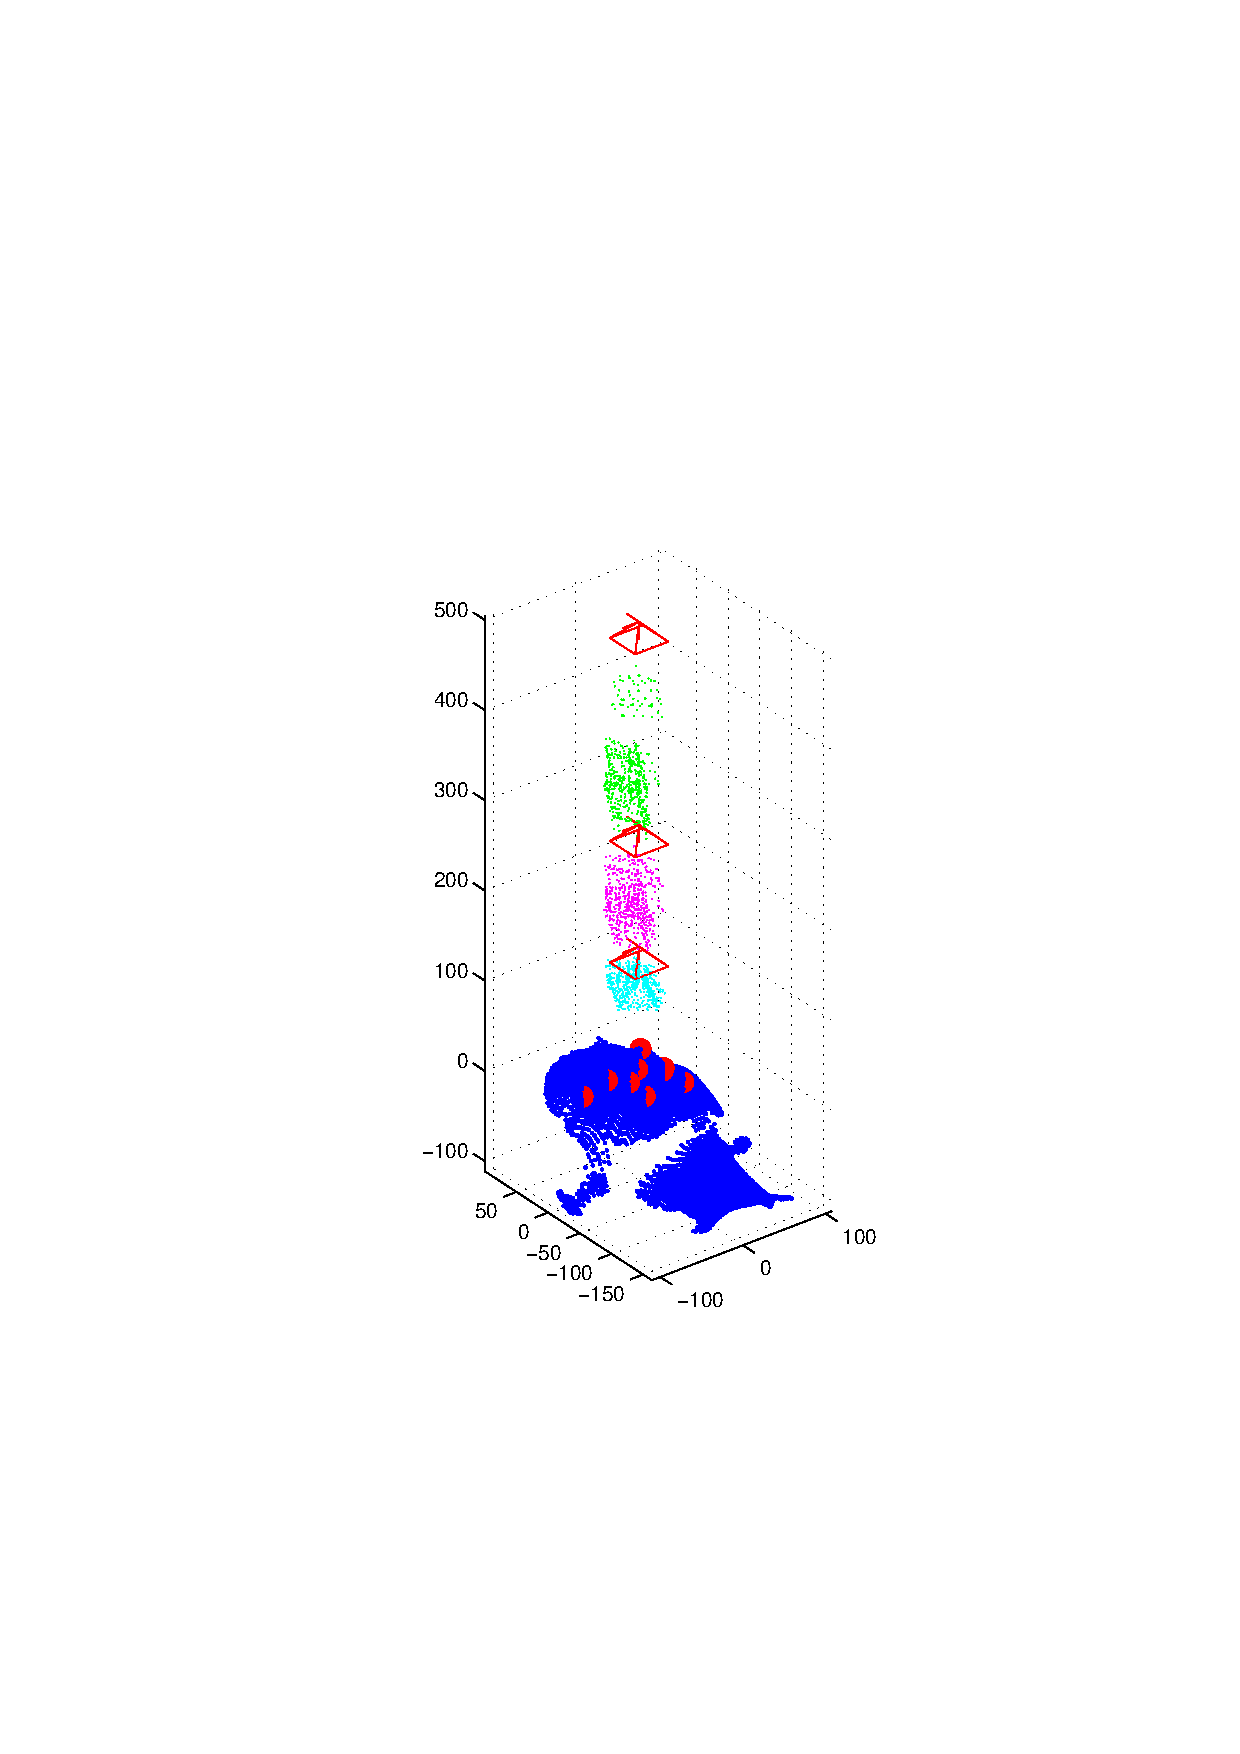
\includegraphics[width=.5\linewidth]{resources/figures/cameraloc_frontal.png} &
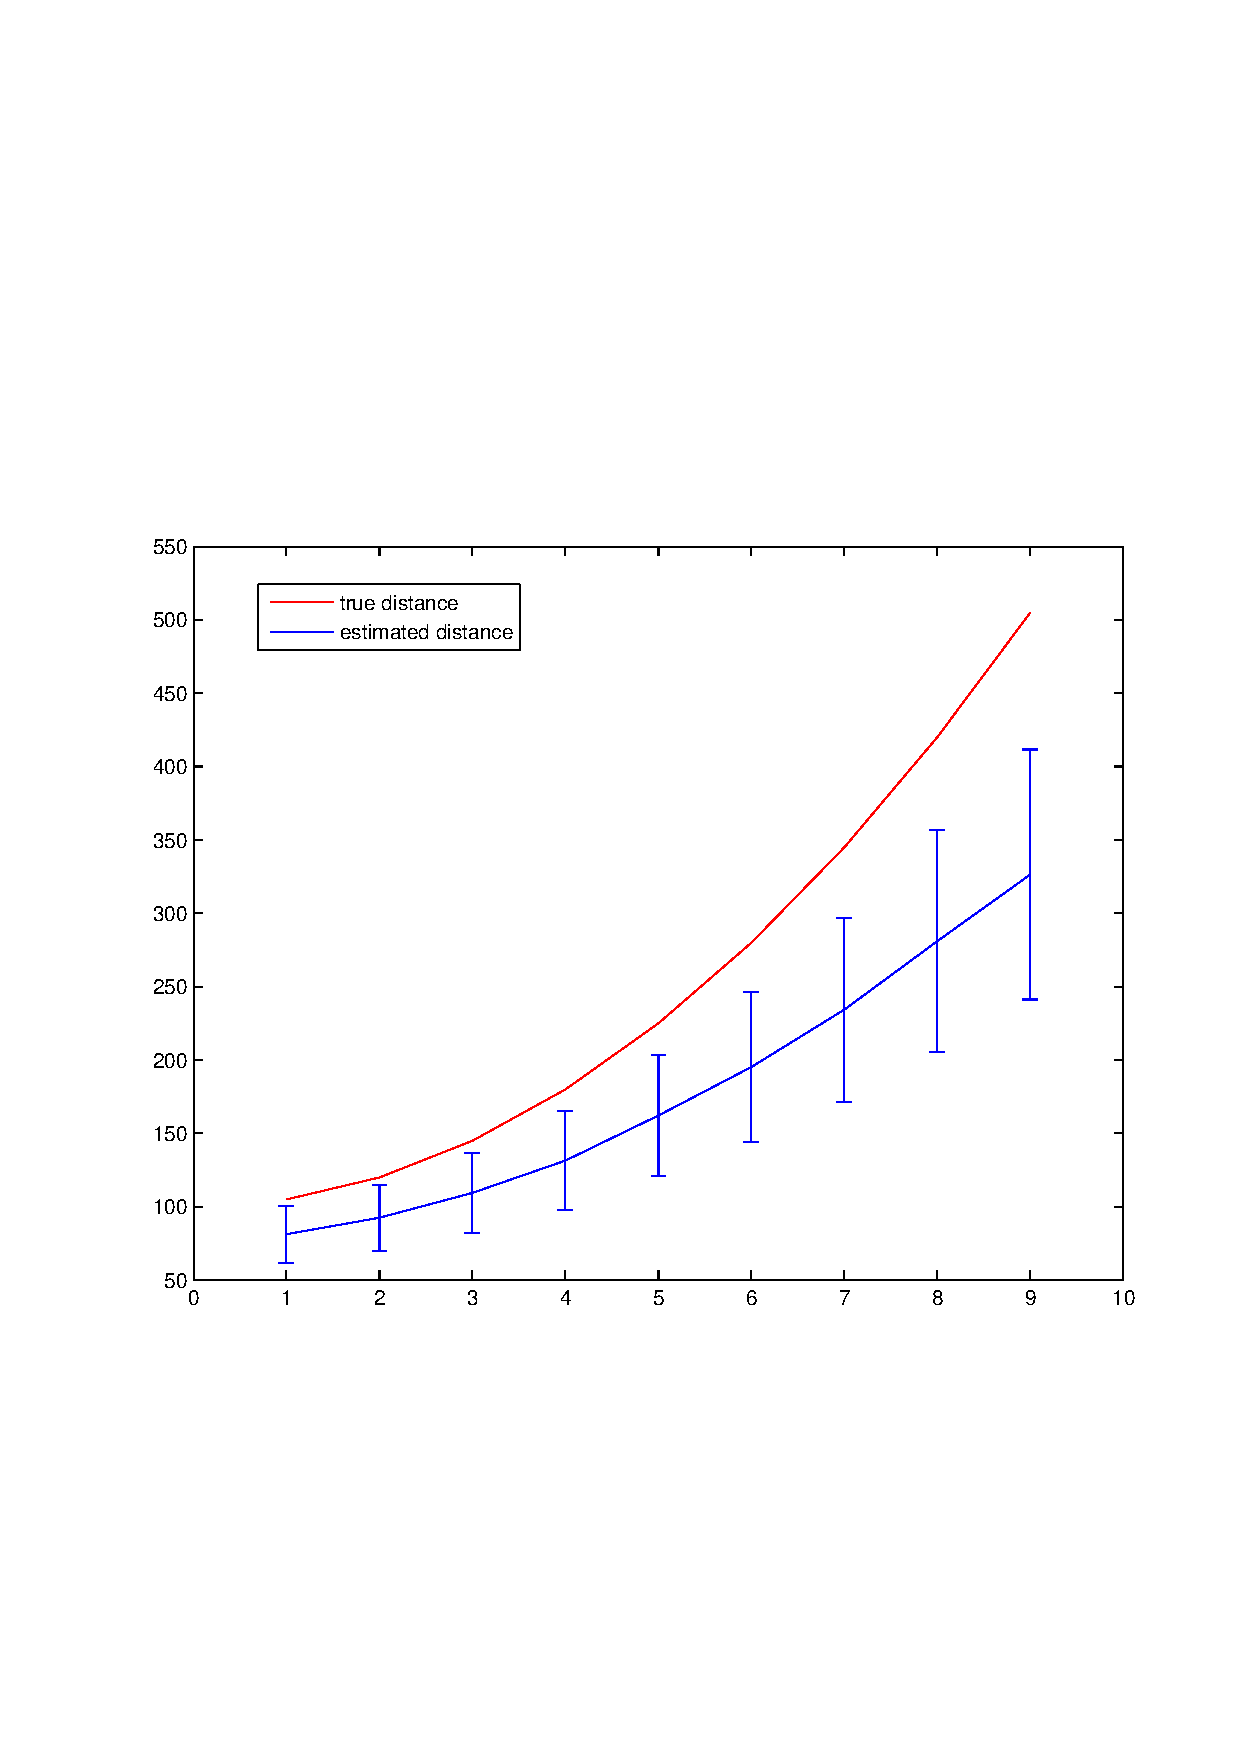
\includegraphics[width=.5\linewidth]{resources/figures/errorbar_frontal.png} \\
(a) & (b) \\
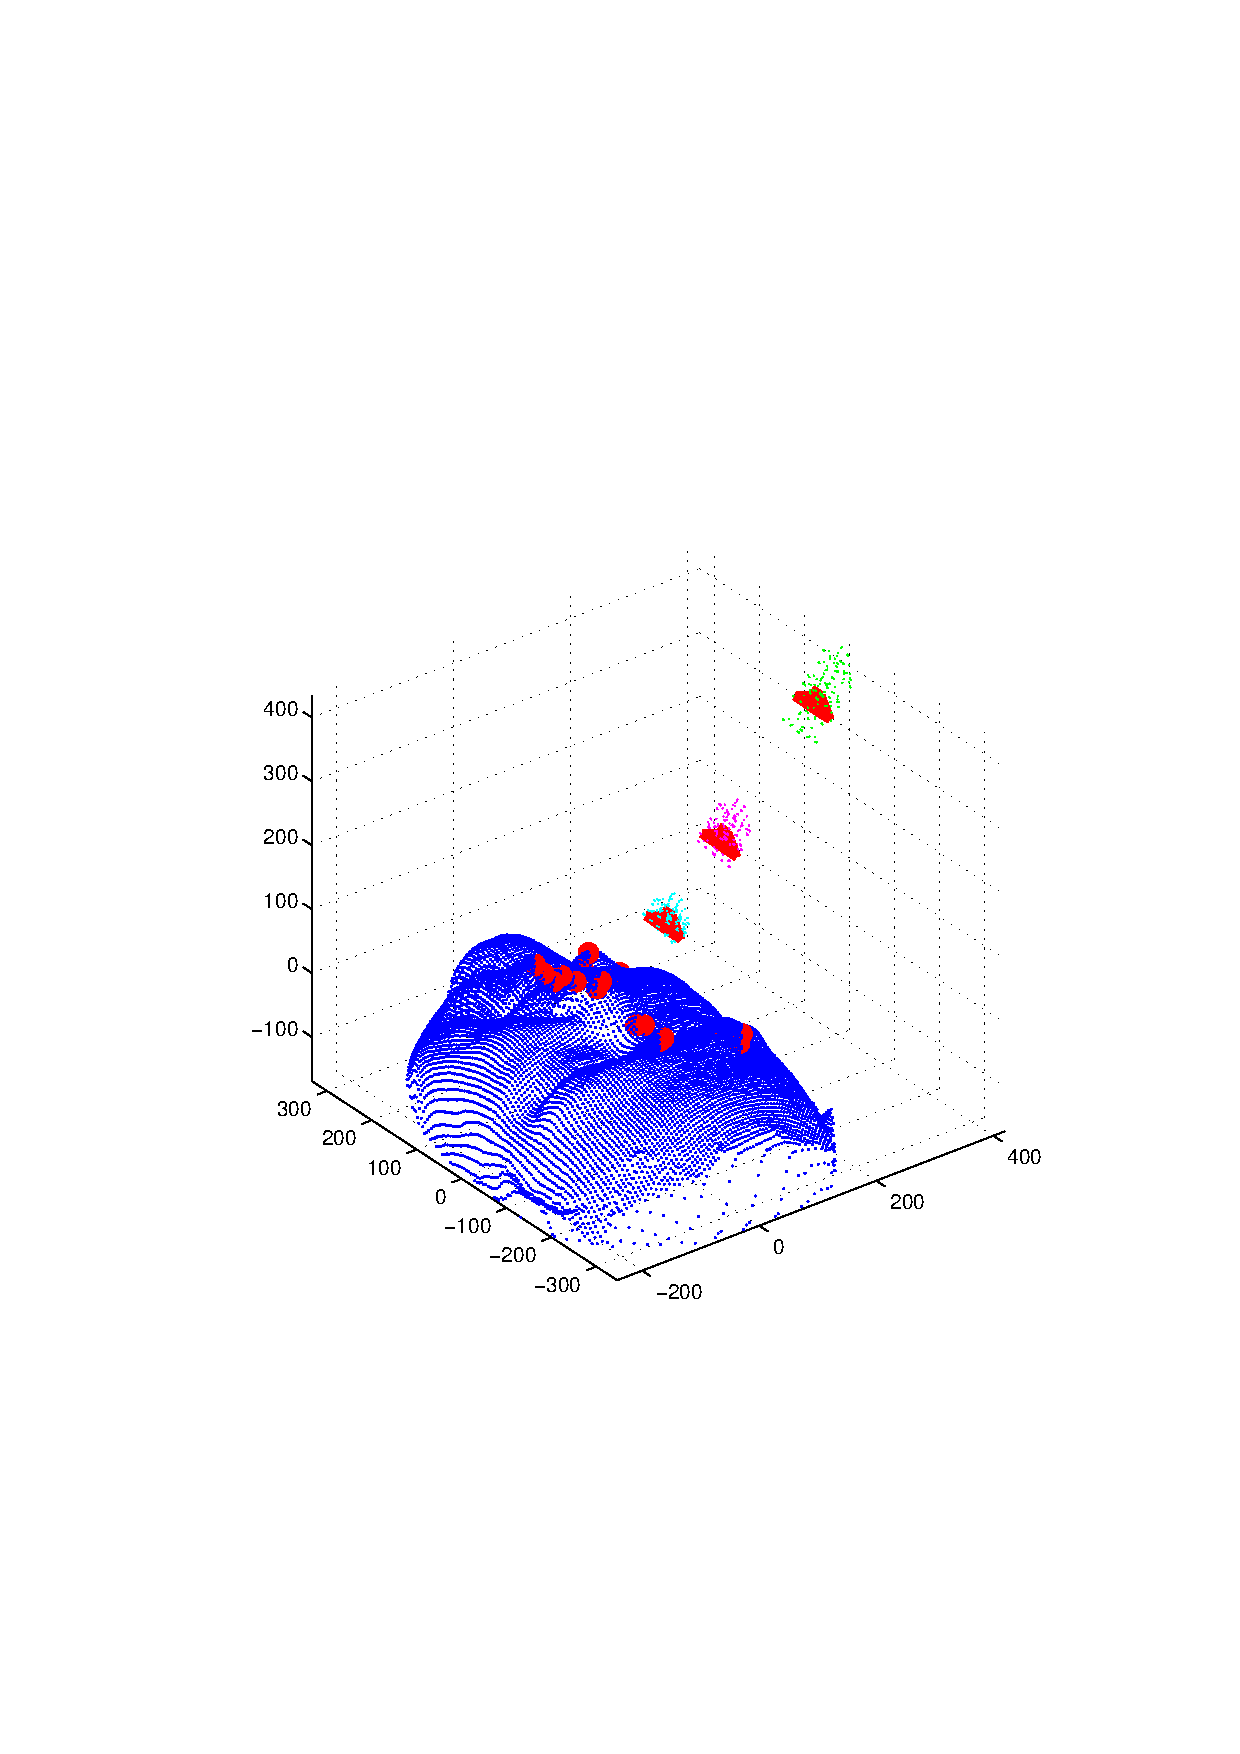
\includegraphics[width=.5\linewidth]{resources/figures/cameraloc_3q.png} &
\includegraphics[width=.5\linewidth]{resources/figures/errorbar_3q.png} \\
(c) & (d)
\end{tabular}
\caption{	
(a) Camera pose estimation results for the frontal case.  
True camera position is the solid red axis.  
Estimated camera positions for near/medium/far are shown in cyan/magenta/green respectively.   
(b) Distance estimate as an average of exemplar models.  
We test $20$ camera positions and corresponding focal length to keep distance between outermost fiducials next to eye at a near constant. 
(c) and (d) show equivalent results for $3/4$ profile view.}
\label{fig:results}
\end{figure}

Figure \ref{fig:error_bar_frontal_lessfiducials} shows the same experiment with different numbers of fiducials used in the \EPnP algorithm.  For this experiment, we manually selected the fiducial subsets to be evenly distributed about the face.  This figure shows the distance can be reliably estimated with as little as $10$ fiducials.  When using only five fiducials, the distance estimate becomes less accurate.  

\begin{figure}[h]
\centering
\includegraphics[width=.7\linewidth]{resources/figures/errorbar_frontal_lessfiducials.png}
\caption{Error bars of camera distance for the frontal view using different numbers of fiducials.}
\label{fig:error_bar_frontal_lessfiducials}
\end{figure}

For qualitative analysis, we use a heuristic to select a ``best'' exemplar.  Let $p_i$ be the 2D imaged fiducial using the true camera position.  
Let $p_{ij}'$ be the imaged fiducial using the estimated camera position from the $j$-th exemplar.
We use $\argmin_j \sum_i \|p_i - p_{ij}'\|$ as a heuristic to select the best exemplar. 
See Figure \ref{fig:bestexemplar} for some illustrative examples.  
In these examples, it is interesting to see what can be recovered by simply using fiducial geometry.  
Top row whos best exemplar matches the gender of the probe image.  
Second row shows similar race in two out of three cases.  
In all cases, the general face of the image is recovered.

\begin{figure}[h]
\centering
\begin{tabular}{cc}
\includegraphics[width=.7\linewidth]{resources/figures/best_exemplar1.png} \\
\includegraphics[width=.7\linewidth]{resources/figures/best_exemplar3.png} \\
\includegraphics[width=.7\linewidth]{resources/figures/best_exemplar10.png} \\
\includegraphics[width=.7\linewidth]{resources/figures/best_exemplar26.png}
\end{tabular}
\caption{Best exemplar face using a simple heuristic.}
\label{fig:bestexemplar}
\end{figure}

\section{Conclusion and future work}
We have shown a method for estimating the distance from camera to a previously unseen face using correspondences of 2D imaged fiducials to 3D fiducial locations on exemplar heads.  
The distance estimate is accurate in distances ranging from 10cm to 300 cm for the frontal and $3/4$ profile views.  
Providing an estimate of this distance can be used to mitage the effects of perspective distortion in face recognition.  

In this paper, we have used a dataset consisting of facial range images with manually labelled fiducials.    
Furthermore we assume an ideal pinhole camera model and we control the pose of both head and camera.  
This simplifies the problem since we have accurate ground truth 2D and 3D fiducial locations. 
For future work, we plan to use methods for detecting fiducials such as \cite{belhumeur2011localizing}.    

\bibliographystyle{splncs}
\bibliography{library}

\end{document}
